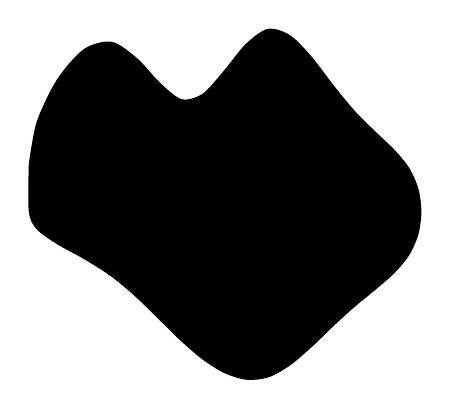
\begin{tikzpicture}[yscale=.6]%[width=\marginparwidth+25pt]
%\begin{axis}[width=\marginparwidth+25pt,%
%tick label style={font=\scriptsize},axis y line=middle,axis x line=middle,name=myplot,axis on top,%
%			%x=.37\marginparwidth,
%			%y=.37\marginparwidth,
%			xtick={1,2,3,4,5,6,7,8,9,10,11,12},% 
%%			extra x ticks={12.57},
%%			extra x tick labels={$4\pi$},
%%			ytick=\empty,
%			%minor y tick num=1,%extra y ticks={-5,-3,...,7},%
%%			minor x tick num=4,
%			ymin=-.1,ymax=8.5,%
%			xmin=-.1,xmax=12.5%
%]

\draw [{\colorone},thick,fill={\coloronefill},smooth] plot coordinates {(0,1.)(0.1013,1.899)(0.3567,2.785)(0.6934,3.42)(1.039,3.569)(1.355,3.224)(1.646,2.705)(1.925,2.355)(2.2,2.473)(2.475,2.968)(2.75,3.529)(3.025,3.844)(3.3,3.709)(3.575,3.249)(3.85,2.651)(4.125,2.098)(4.389,1.661)(4.624,1.285)(4.807,0.9071)(4.921,0.4743)(4.958,0)(4.921,-0.4743)(4.807,-0.9071)(4.624,-1.279)(4.389,-1.625)(4.125,-1.986)(3.85,-2.401)(3.575,-2.843)(3.3,-3.233)(3.025,-3.487)(2.75,-3.536)(2.475,-3.397)(2.2,-3.111)(1.925,-2.718)(1.646,-2.263)(1.355,-1.792)(1.039,-1.352)(0.6934,-0.9844)(0.3567,-0.6744)(0.1013,-0.3653)(0,0)(0,1)};

\draw (1,3.56) -- (1,-1.35) node [shift={(-3pt,0pt)},rotate=90,pos=.5] {\scriptsize 4.9};

\draw (2,2.37) -- (2,-2.8) node [shift={(-3pt,0pt)},rotate=90,pos=.5] {\scriptsize 5.2};

\draw (3,3.8) -- (3,-3.5) node [shift={(-3pt,0pt)},rotate=90,pos=.5] {\scriptsize 7.3};

\draw (4,2.35) -- (4,-2.15) node [shift={(-3pt,0pt)},rotate=90,pos=.5] {\scriptsize 4.5};

%\end{axis}
%
%\node [right] at (myplot.right of origin) {\scriptsize $x$};
%\node [above] at (myplot.above origin) {\scriptsize $y$};
\end{tikzpicture}


